% !TEX root = SegwayDoku.tex
\newpage
\renewcommand{\autoren}{Valentyn Chepil}
\section{Das Gehäuse}
\subsection{Das Gehäuse - V.1}
% \ref{bild_3} zuweisung auf Bild in Text.
\begin{figure}[!h]  % [h] bedeutet, dass das Bild genau an dieser Stelle im Text erscheint
	% mit width=... wird die Größe des Bildes in Prozent der Seitenbreite eingestellt
	\centering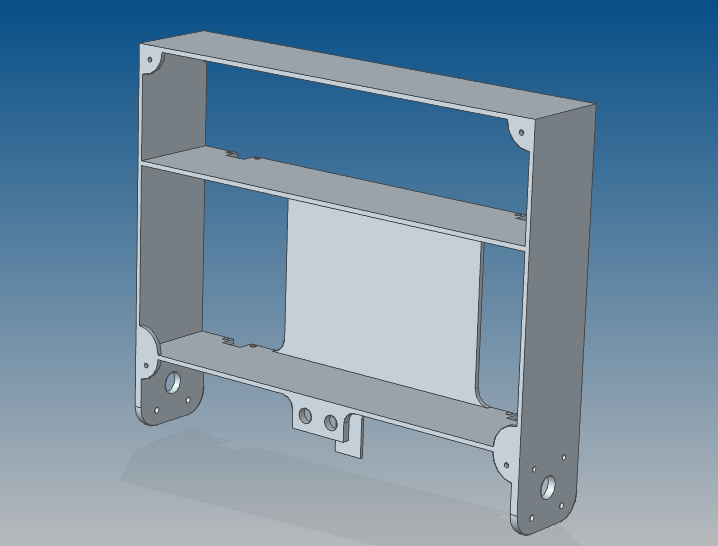
\includegraphics[width=0.5\textwidth]{images/gehaeuse-v1.png}
	% caption ist die Bildunterschrift, taucht auch im Abbildungsverzeichnis auf
	\caption{Das Gehäuse - V.1 \newline (Quelle: eigene Darstellung)}
	\label{gehaeuse-v1} % über das label kann man aus dem Text auf das Bild verweisen
\end{figure}
Gefordert wurde ein einfacher Aufbau des Gehäuses in Kastenform.
\subsection{Das Gehäuse - V.2}
\begin{figure}[!h]  % [h] bedeutet, dass das Bild genau an dieser Stelle im Text erscheint
	% mit width=... wird die Größe des Bildes in Prozent der Seitenbreite eingestellt
	\centering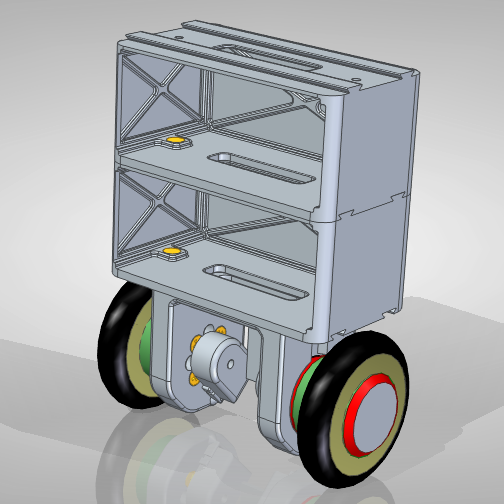
\includegraphics[width=0.5\textwidth]{images/gehaeuse-v2.png}
	% caption ist die Bildunterschrift, taucht auch im Abbildungsverzeichnis auf
	\caption{Das Gehäuse - V.2 \newline (Quelle: eigene Darstellung)}
	\label{gehaeuse-v2} % über das label kann man aus dem Text auf das Bild verweisen
\end{figure}
Im Bild \ref{gehaeuse-v2} ist eine modulare Darstellung des Roboters zu sehen. Der Motorhalter ist in diesem Fall als ein externes Modul dargestellt. Das oberste Modul ist für die Steuerungsplatinen vorgesehen. Im zweiten Modul von oben sollte  der Akku verbaut werden. Mit Hilfe von Schwalbenschwanzverbindungen und zwei Schrauben sollten die Module miteinander verbunden werden.

\subsection{Das Gehäuse - V.3}

Die Version V.2 (Bild \ref{gehaeuse-v2}) unterscheidet sich nicht viel von V.3. Es wurde am modularen Aufbau nichts verändert. Jedoch haben wir die Schwalbenschwanzverbindungen durch Steckverbindungen ersetzt, die seitlich Zugeordnet sind. Es wurde auch der Motorhalter modifiziert.

\begin{figure}[!h]  % [h] bedeutet, dass das Bild genau an dieser Stelle im Text erscheint
	% mit width=... wird die Größe des Bildes in Prozent der Seitenbreite eingestellt
	\centering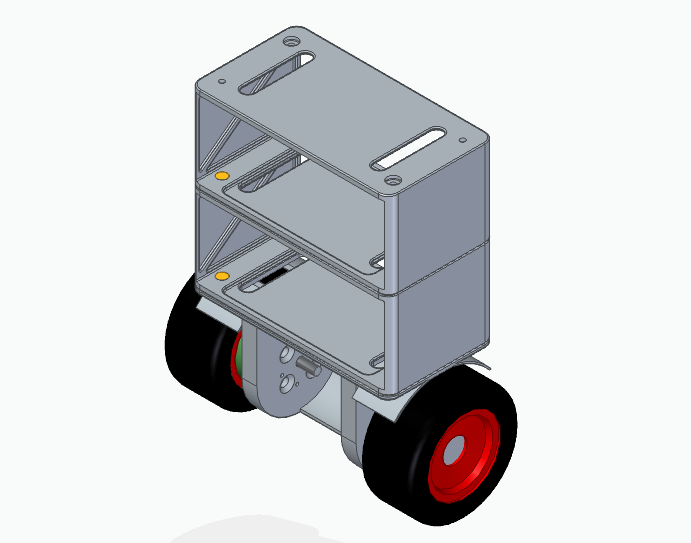
\includegraphics[width=0.5\textwidth]{images/gehaeuse-v3.png}
	% caption ist die Bildunterschrift, taucht auch im Abbildungsverzeichnis auf
	\caption{Das Gehäuse - V.2 \newline (Quelle: eigene Darstellung)}
	\label{gehaeuse-v3} % über das label kann man aus dem Text auf das Bild verweisen
\end{figure}

\subsection{Das Gehäuse - V.4}

Das endgültige Gehäuse ist auf der Abbildung \ref{gehaeuse-v4} zu betrachten. Diese Version wurde durch sintern hergestellt.

\begin{figure}[htb]
	\centering
	\begin{minipage}{0.45\linewidth}
		\centering
		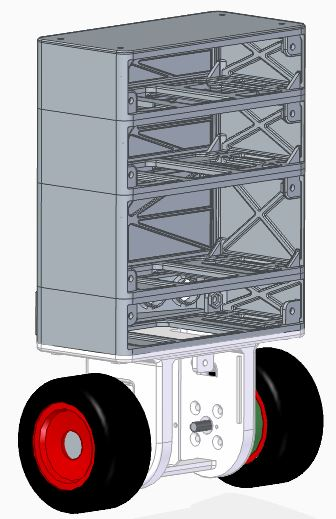
\includegraphics[scale=0.48]{images/4.1_vorne.jpg}
		\caption{Endgültiges Gehäuse V4.1 \newline(Quelle: Eigene Darstellung)}
		\label{gehaeuse-v4}
	\end{minipage}
	%\hfill
	\begin{minipage}{0.45\linewidth}
		\centering
		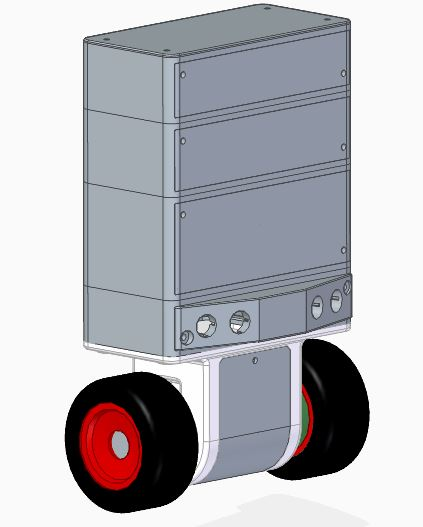
\includegraphics[scale=0.48]{images/4.1_hinten.jpg}
		\caption{ mit Deckels \newline (Quelle: Eigene Darstellung)}
	\end{minipage}
\end{figure}
\pagebreak
\subsection{Das Gehäuse - V.4.2.3}

Nach Zusammenbau des Roboters wurden folgende Korrekturen noch durchgeführt:
 
\begin{itemize} 
	\item  mBed-Modul wurde 10 mm höher gesetzt.
	\item  Anpassung an Kabelkanal Führung.
	\item  Beschriftung der Module.
	\item  Oberwand wurde komplett entfernt.
	\item  Versteifungen als Deckelsturzstelle.
	\item  Akku-Modul wurde 10 mm höher gesetzt.
	\item  mBed und oDrive wurden stark nach einer Seite platziert.
\end{itemize}

\begin{figure}[htb]
	\centering
	\begin{minipage}{0.45\linewidth}
		\centering
		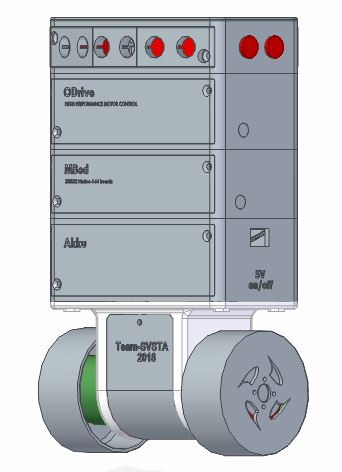
\includegraphics[scale=0.48]{images/V.4.3.jpg}
		\caption{Gehäuse V4.3 \newline(Quelle: Eigene Darstellung)}
		\label{gehaeuse-v4.3}
	\end{minipage}
	%\hfill
	\begin{minipage}{0.45\linewidth}
		\centering
		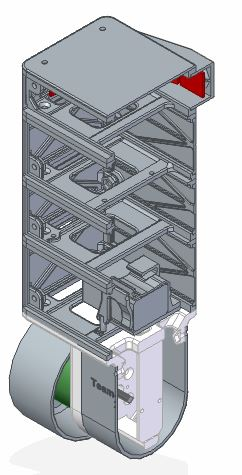
\includegraphics[scale=0.48]{images/V.4.3-1.jpg}
		\caption{ Schnitt \newline (Quelle: Eigene Darstellung)}
	\end{minipage}
\end{figure}

\subsubsection{ Berechnung vom Motorträger}
Alle Berechnungen wurden mit Hilfe von FEM - Programmierung erstellt und beweisen die Festigkeit vom Motorhalter. An den  Motor bzw. und Radstellen wurde das Moment laut der Berechnung \ref{FEM1} verwendet. Des Weiteren wurde eine Lastkraft von 50N auf die Oberfläche eingeprägt.

Die Materialeigenschaften kann man aus der Abbildung \ref{FEM2} ablesen.
\pagebreak
\begin{figure}[!h]  % [h] bedeutet, dass das Bild genau an dieser Stelle im Text erscheint
	\centering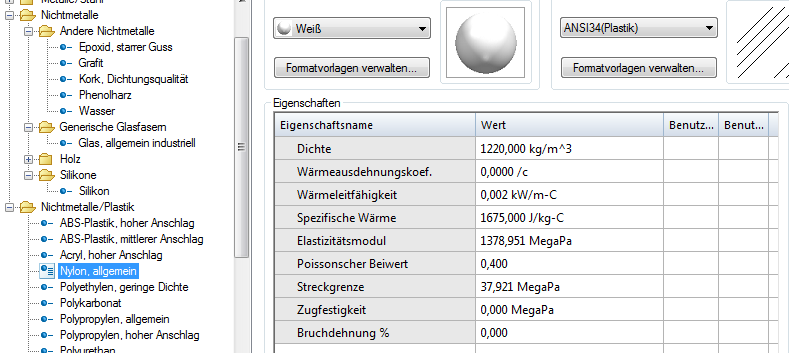
\includegraphics[width=0.7\textwidth]{images/FEM2.png}
	% caption ist die Bildunterschrift, taucht auch im Abbildungsverzeichnis auf
	\caption{Kunststoffeigenschaften - Nylon (PA) \newline (Quelle: eigene Darstellung)}
	\label{FEM2} % über das label kann man aus dem Text auf das Bild verweisen
\end{figure}

Der Motorträger wurde minimal vernetzt, um die Berechnungszeit zu reduzieren.

\begin{figure}[!h] 
	\centering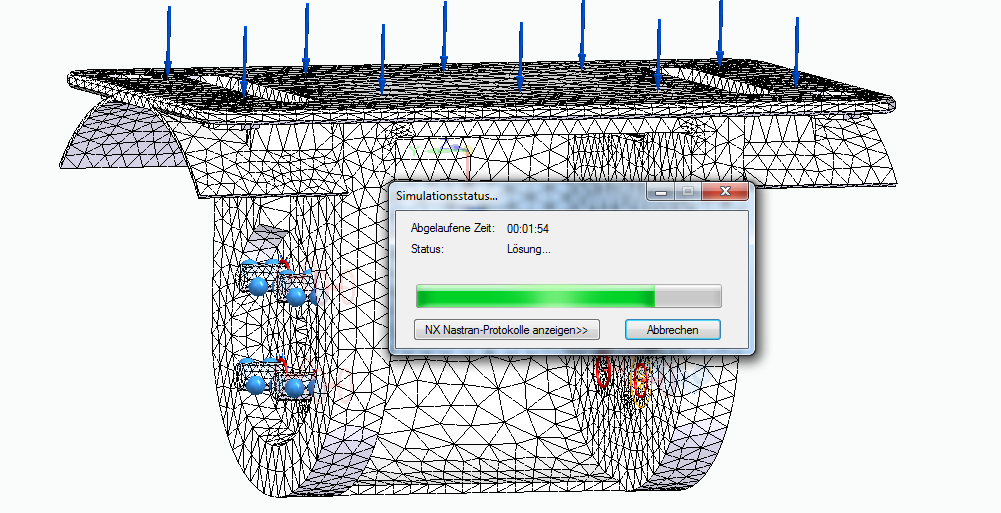
\includegraphics[width=0.8\textwidth]{images/FEM.png}
	\caption{FEM-Berechnung \newline (Quelle: eigene Darstellung)}
	\label{FEM1} % über das label kann man aus dem Text auf das Bild verweisen
\end{figure}

Die Verschiebungen und Spannungen sind auf den Bildern \ref{FEM3} und \ref{FEM4} zu sehen. 

\begin{figure}[htb]
	\centering
	\begin{minipage}{0.49\linewidth}
		\centering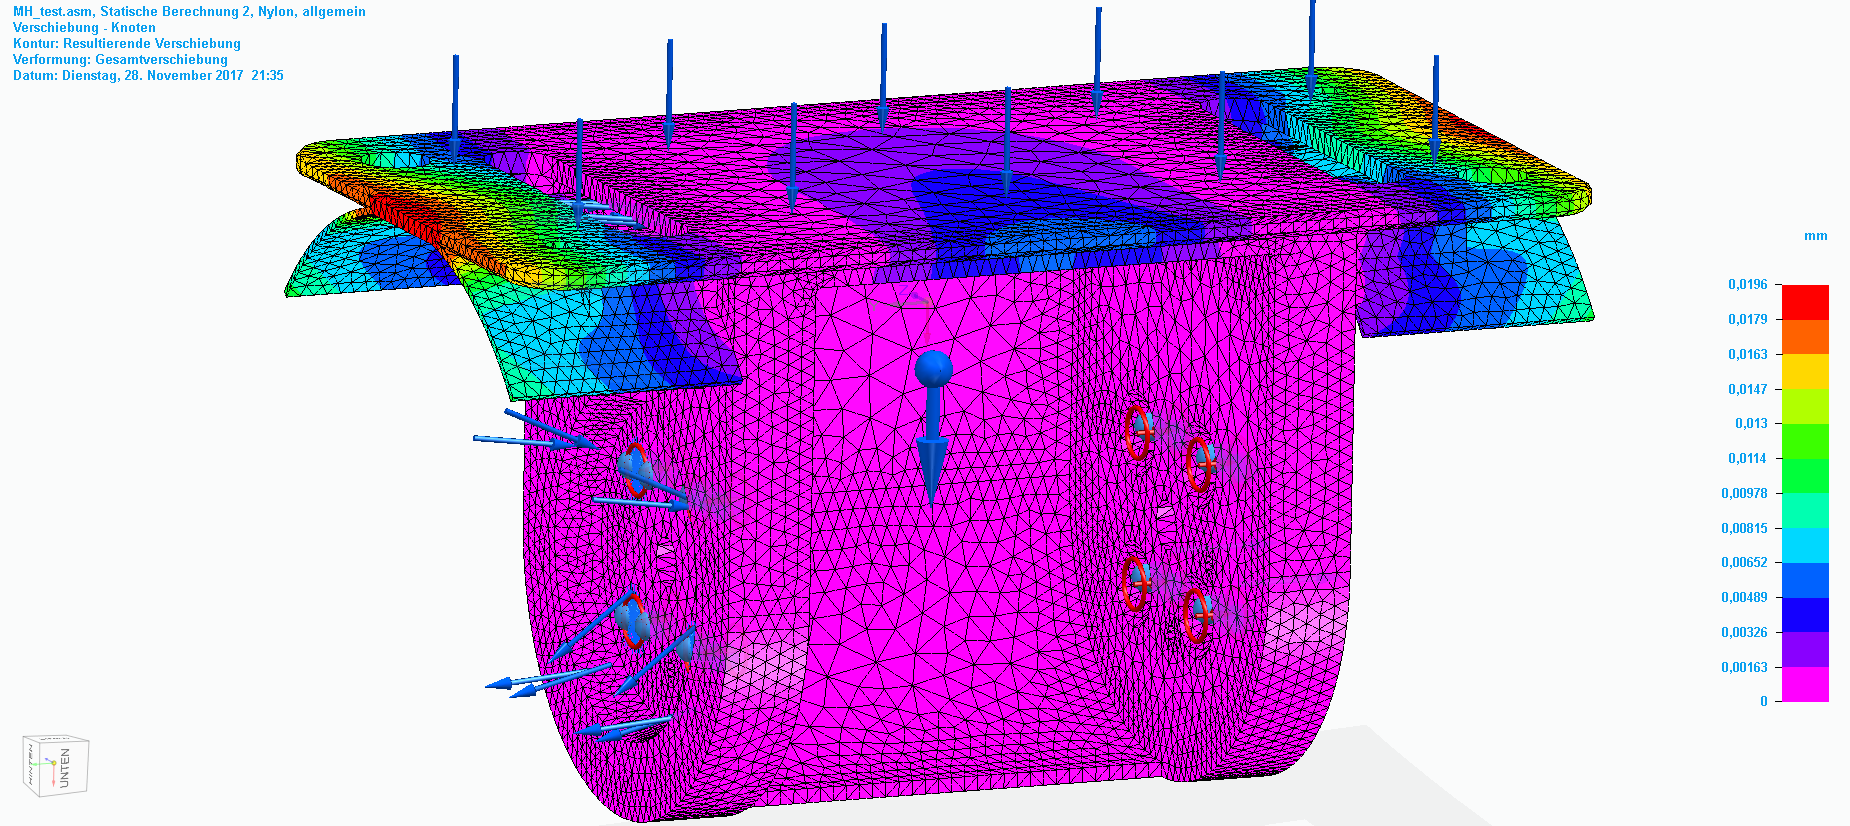
\includegraphics[width=0.9\textwidth]{images/FEM3.png}
		\caption{FEM - Verschiebungen \newline (Quelle: eigene Darstellung)}
		\label{FEM3}
	\end{minipage}
	\begin{minipage}[h]{0.49\linewidth}
		\centering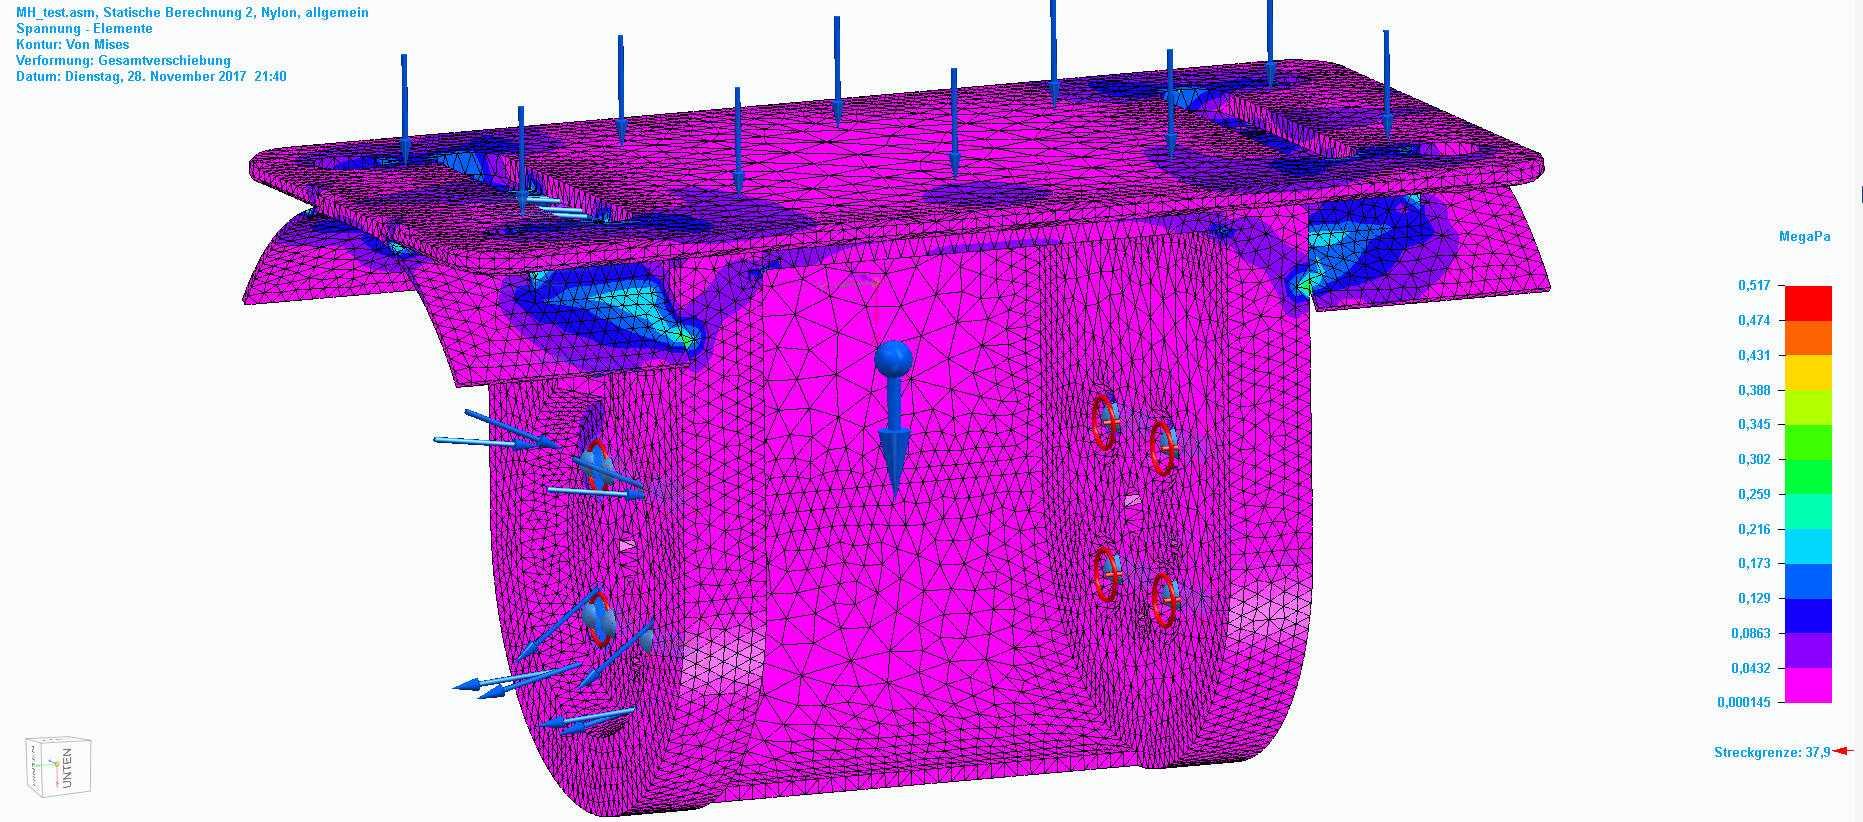
\includegraphics[width=0.9\textwidth]{images/FEM4.png}
		\caption{FEM - Spannungen \newline (Quelle: eigene Darstellung)}
		\label{FEM4}
	\end{minipage}
\end{figure}

Auf den Abbildungen \ref{FEM3}, \ref{FEM4} ist zu sehen, dass der Sicherheitsfaktor des Motorträgers deutlich höher als 2 ist und somit keine weiteren Berechnungen nötig sind.

